\documentclass{beamer}
\usetheme[faculty=ped,basePath=../fibeamer,logo=../fibeamer/logo/mu/Logo-UC-3.png]{fibeamer}
\graphicspath{{../resources/}}

\usepackage{algorithm}
\usepackage{algpseudocode}

\usetheme[faculty=ped]{fibeamer}
\usepackage[utf8]{inputenc}
\usepackage[
  main=english, %% By using `czech` or `slovak` as the main locale
                %% instead of `english`, you can typeset the
                %% presentation in either Czech or Slovak,
                %% respectively.
  czech, slovak %% The additional keys allow foreign texts to be
]{babel}        %% typeset as follows:
%%
%%   \begin{otherlanguage}{czech}   ... \end{otherlanguage}
%%   \begin{otherlanguage}{slovak}  ... \end{otherlanguage}
%%
%% These macros specify information about the presentation
\title{Recursividad} %% that will be typeset on the
\subtitle{Semestre II-2026} %% title page.
\author{Profesora: Andreina Cota Vidaurre}
%% These additional packages are used within the document:
\usepackage{ragged2e}  % `\justifying` text
\usepackage{booktabs}  % Tables
\usepackage{tabularx}
\usepackage{tikz}      % Diagrams
\usetikzlibrary{calc, shapes, backgrounds}
\usetikzlibrary{positioning, arrows.meta, shadows.blur, shapes.geometric}
\usepackage{amsmath, amssymb}
\usepackage{url}       % `\url`s
\usepackage{listings}  % Code listings
\usepackage{graphicx}
\usepackage{amsmath}
\usepackage[T1]{fontenc}
\usepackage{xcolor}
\usepackage{minted}
% \usepackage{adjustbox}


% Definicion de pseudocodigo en espaniol
\lstdefinelanguage{PseudocodigoES}{
    morekeywords={INICIO,FIN,PARA,HACER,SI,ENTONCES,FIN_SI,FIN_PARA,IMPRIMIR},
    sensitive=true,
    morecomment=[l]{//},
    morestring=[b]"
}

% Definicion de pseudocodigo en ingles
\lstdefinelanguage{PseudocodeEN}{
    morekeywords={BEGIN,END,FOR,DO,IF,THEN,END_IF,END_FOR,PRINT},
    sensitive=true,
    morecomment=[l]{//},
    morestring=[b]"
}

\lstset{
    basicstyle=\ttfamily\small,
    keywordstyle=\bfseries,
    columns=fullflexible,
    keepspaces=true,
    showstringspaces=false,
    frame=single,
    xleftmargin=0em,
    framexleftmargin=0em,
    framesep=2pt,
    gobble=4,
    resetmargins=true,
    aboveskip=0pt,
    belowskip=0pt
}

\lstdefinestyle{pythonstyle}{
    language=Python,
    basicstyle=\ttfamily\small,
    keywordstyle=\bfseries,
    commentstyle=\itshape,
    stringstyle=\ttfamily,
    showstringspaces=false,
    columns=fullflexible,
    keepspaces=true,
    frame=single,
    breaklines=true,
    xleftmargin=0em,
    framexleftmargin=0em,
    framesep=2pt,
    aboveskip=0pt,
    belowskip=0pt,
    gobble=4,
    resetmargins=true,
    emph={print,input,int,float,str,bool,len,range},
    emphstyle=\bfseries
}

\lstset{style=pythonstyle}

% Estilos del diagrama
\tikzstyle{iniciofin} = [
    ellipse,
    minimum width=2.5cm,
    minimum height=1cm,
    text centered,
    draw=black,
    fill=blue!25
]

\tikzstyle{proceso} = [
    rectangle,
    rounded corners,
    minimum width=3cm,
    minimum height=1cm,
    text centered,
    draw=black,
    fill=cyan!20
]

\tikzstyle{decision} = [
    diamond,
    aspect=2,
    text centered,
    draw=black,
    fill=yellow!35
]

\tikzstyle{flecha} = [
    thick,
    ->,
    >=Stealth
]


\frenchspacing
\begin{document}
  \shorthandoff{-}
  \frame[c]{\maketitle}

    \begin{frame}{Contenido}
        \begin{itemize}
            \item Introducción
            \item Fundamentos
            \item Funcionamiento interno
            \item Ejemplos
            \item Diferencias entre recursividad e iteración
            \item Cuándo utilizar recursividad?
            \item Ventajas y desventajas
            \item Ejercicios
            \item Resumen
        \end{itemize}
    \end{frame}

    \begin{frame}{Introducción}
        \textcolor{blue}{\textbf{Cómo calcular el factorial de un número sin usar iteraciones?}}
    \end{frame}

    \begin{frame}{Introducción}
        \textcolor{blue}{\textbf{Cómo calcular el factorial de un número sin usar iteraciones?}}

        El factorial de un número se puede calcular de la siguiente manera:
        \begin{equation}
            n! = n \times (n-1)!
        \end{equation}
    \end{frame}

    \begin{frame}{Introducción}
        \setcounter{equation}{0}
        \textcolor{blue}{\textbf{Cómo calcular el factorial de un número sin usar iteraciones?}}

        El factorial de un número se puede calcular de la siguiente manera:
        \begin{equation}
            n! = n \times (n-1)!
        \end{equation}
        Descomponiendo el factorial en factores más pequeños:
        \begin{equation}
            n! = n \times (n-1) \times (n-2) \times \cdots \times 1
        \end{equation}
        Caso base:
        \begin{equation}
            0! = 1
        \end{equation}
    \end{frame}

    \begin{frame}{Introducción}
        \textcolor{blue}{\textbf{Es posible resolver un problema utilizando una versión más pequeña del mismo problema?}}    
    \end{frame}

    \begin{frame}{Recursividad}
        \begin{itemize}
            \item Es una técnica de programación que permite resolver un problema mediante 
            llamadas a una función que resuelve versiones más pequeñas del mismo problema.
            \item Una función recursiva es una función que se llama a sí misma.
        \end{itemize}
    \end{frame}

    \begin{frame}{Fundamentos}
        \textcolor{blue}{\textbf{Qué necesita una función recursiva para llamarse a sí misma sin ejecutarse indefinidamente?}}
        \begin{enumerate}
            \item \textbf{Caso base}: Condición que permite terminar la recursividad sin realizar otra llamada recursiva.
            \item \textbf{Caso recursivo}: Parte de la función que realiza una nueva llamada para resolver un subproblema.
            \item \textbf{Llamada recursiva}: Es la llamada que debe acercar el problema al caso base.
        \end{enumerate}
    \end{frame}

    \begin{frame}[fragile, t]{Fundamentos}
        Ejemplo: Función que imprime una cuenta regresiva desde un número hasta 0. Al llegar a 0, imprime \mintinline{python}{"Happy Halloween!"}.
        \begin{minted}[xleftmargin=-2cm, frame=leftline, fontsize=\small]{python}
            def cuenta_regresiva(n):
                # Caso base
                if n == 0:
                    print("Happy Halloween!")
        \end{minted}
    \end{frame}

    \begin{frame}[fragile, t]{Fundamentos}
        Ejemplo: Función que imprime una cuenta regresiva desde un número hasta 0. Al llegar a 0, imprime \mintinline{python}{"Happy Halloween!"}.
        \begin{minted}[xleftmargin=-2cm, frame=leftline, fontsize=\small]{python}
            def cuenta_regresiva(n):
                # Caso base
                if n == 0:
                    print("Happy Halloween!")
                # Caso recursivo
                else:
                    print(n) 
                    # Llamada recursiva
                    cuenta_regresiva(n-1) 
        \end{minted}
    \end{frame}

    \begin{frame}[fragile, t]{Fundamentos}
        Ejemplo: Función que calcula el factorial de un número.
        \begin{minted}[xleftmargin=-2cm, frame=leftline, fontsize=\small]{python}
            def factorial(n):
                resultado = Nan
                # Caso base
                if n == 0:
                    resultado = 1
                return resultado
        \end{minted}
    \end{frame}

    \begin{frame}[fragile, t]{Fundamentos}
        Ejemplo: Función que calcula el factorial de un número.
        \begin{minted}[xleftmargin=-2cm, frame=leftline, fontsize=\small]{python}
            def factorial(n):
                resultado = Nan
                # Caso base
                if n == 0:
                    resultado = 1
                # Caso recursivo
                else:
                    resultado = n * factorial(n-1)
                return resultado
        \end{minted}
    \end{frame}

    \begin{frame}[fragile, t]{Fundamentos}
        Ejemplo: Función que calcula el factorial de un número.

        \textcolor{blue}{\textbf{Qué sucede cuando no existe el caso base?}}
        \begin{minted}[xleftmargin=-2cm, frame=leftline, fontsize=\small]{python}
            def factorial(n):
                # Caso recursivo
                resultado = n * factorial(n-1)
                return resultado
        \end{minted}
    \end{frame}

    \begin{frame}[fragile, t]{Funcionamiento interno}
        \begin{itemize}
            \item Cuando una función se llama a sí misma, se crea un nuevo espacio en la memoria para la nueva llamada.
            \item Cuando la función llega al caso base, se retorna el valor y se elimina el espacio en la memoria.
        \end{itemize}
    \end{frame}

    \begin{frame}[fragile, t]{Funcionamiento interno}
        Al ejecutar:
        \begin{minted}[xleftmargin=-2cm, frame=leftline, fontsize=\small]{python}
            factorial(3)
        \end{minted}

        Se producen las siguientes llamadas:
        \begin{verbatim}
factorial(3)
  factorial(2)
    factorial(1)
      factorial(0)
        \end{verbatim}
    \end{frame}

    \begin{frame}[fragile, t]{Funcionamiento interno}
        Una vez alcanzado el caso base, se retorna el valor y se elimina el espacio en la memoria.
        
        Existen dos momentos importantes en la ejecución de una función recursiva:
        \begin{itemize}
            \item \textbf{Llamada recursiva}: Reduce el problema hasta alcanzar el caso base.
            \item \textbf{Retorno}: Las llamadas pendientes continúan su ejecución y combinan sus resultados.
        \end{itemize}
    \end{frame}

    \begin{frame}[fragile, t]{Ejemplo: Factorial}
        \begin{align*}
            \mathit{factorial}(3)
                &= 3 \times \mathit{factorial}(2) \\
                &= 3 \times \bigl(2 \times \mathit{factorial}(1)\bigr) \\
                &= 3 \times \bigl(2 \times \bigl(1 \times \mathit{factorial}(0)\bigr)\bigr) \\
                &= 3 \times \bigl(2 \times \bigl(1 \times 1\bigr)\bigr) \\
                &= 3 \times \bigl(2 \times 1\bigr) \\
                &= 3 \times 2 \\
                &= 6
        \end{align*}
    \end{frame}

    \begin{frame}[fragile, t]{Ejemplo: Factorial}
        \begin{figure}
            \centering
            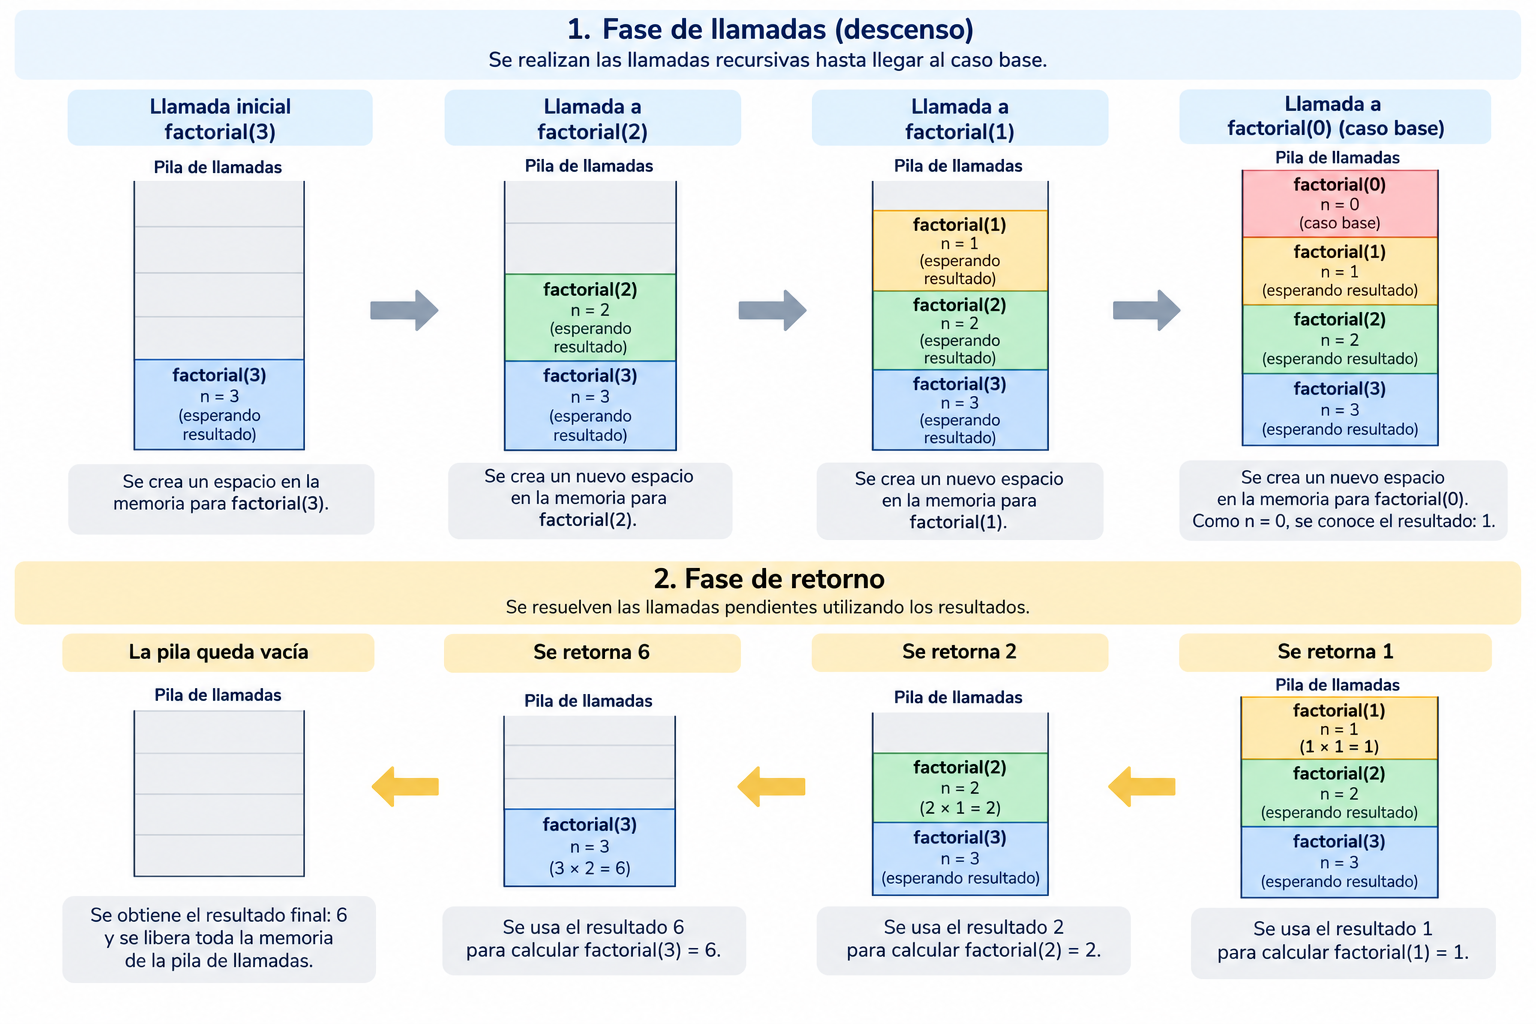
\includegraphics[width=\linewidth]{recursividad_fundamento_simple.png}
        \end{figure}
    \end{frame}

    \begin{frame}[fragile, t]{Ejemplo: Fibonacci}
        \setcounter{equation}{0}
        La secuencia de Fibonacci es una secuencia de números donde cada número es la suma de los dos anteriores.
        \begin{itemize}
            \item 0, 1, 1, 2, 3, 5, 8, 13, 21, 34, 55, 89, 144, ...
        \end{itemize}
        La fórmula para calcular el n-ésimo número de la secuencia es:
        \begin{equation}
            F(n) = F(n-1) + F(n-2)
        \end{equation}

        Caso base:
        \begin{equation}
            F(0) = 0, F(1) = 1
        \end{equation}
    \end{frame}

    \begin{frame}[fragile, t]{Ejemplo: Fibonacci}
        \begin{minted}[xleftmargin=-2cm, frame=leftline, fontsize=\small]{python}
            def fibonacci(n):
                if n == 0:
                    return 0
                elif n == 1:
                    return 1
                else:
                    return fibonacci(n-1) + fibonacci(n-2)
        \end{minted}
    \end{frame}

    \begin{frame}[fragile, t]{Ejemplo: Fibonacci}
        \begin{figure}
            \centering
            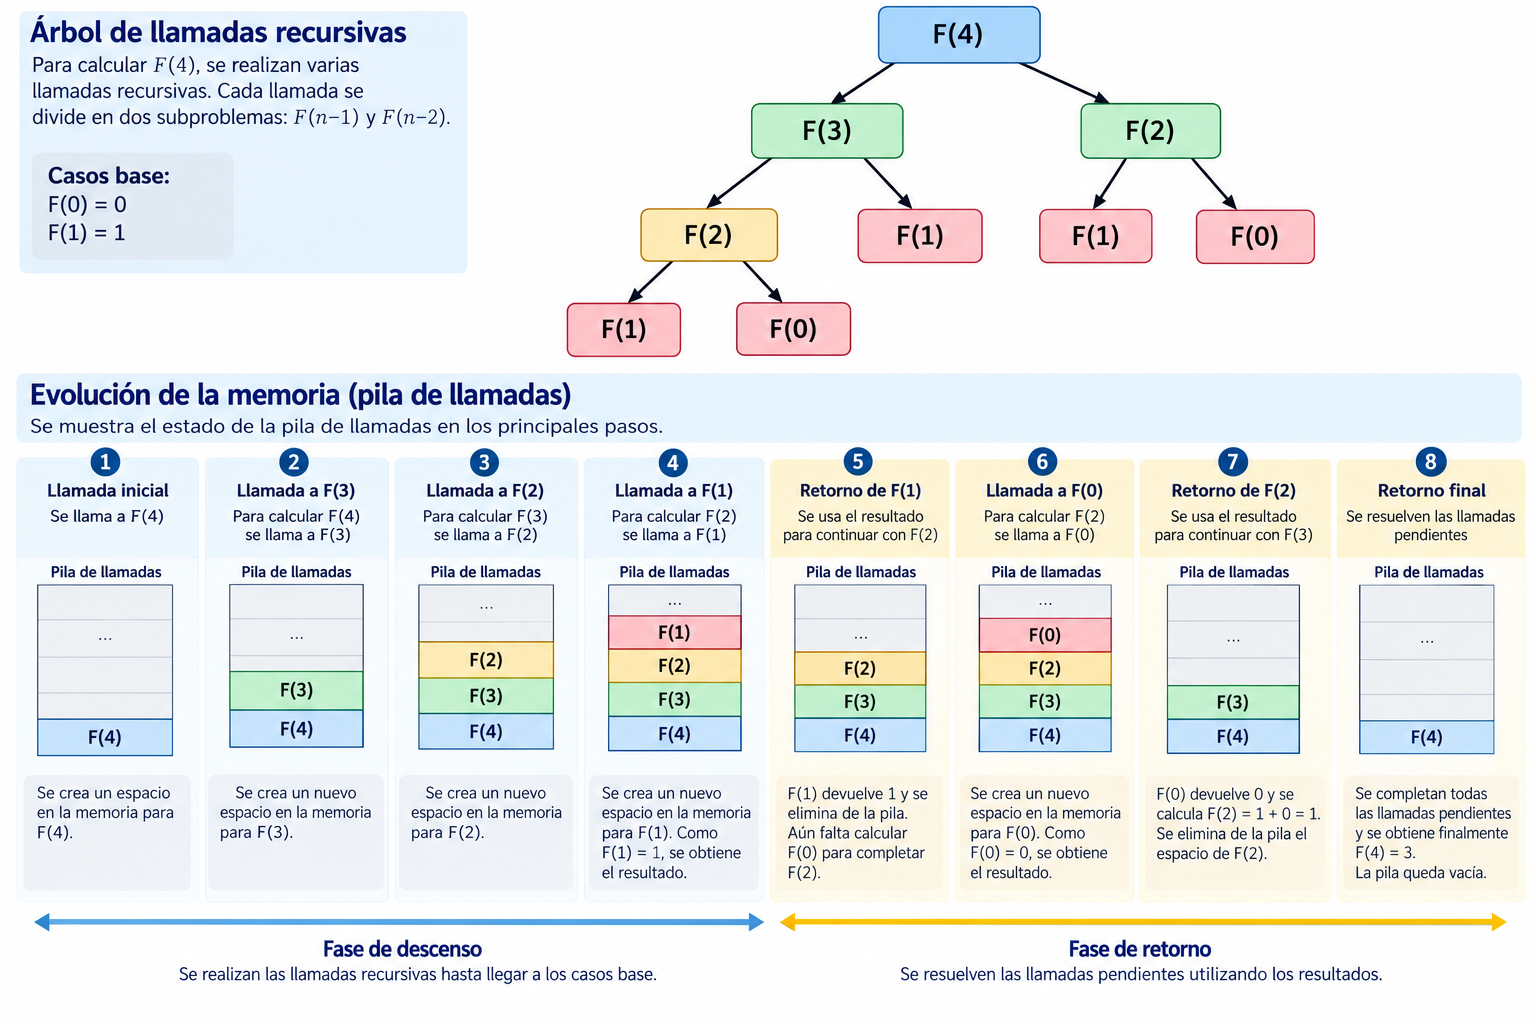
\includegraphics[width=\linewidth]{recursividad_fibonacci.png}
        \end{figure}
    \end{frame}

    \begin{frame}[fragile, t]{Ejemplo: Suma de elementos de una lista}
        Se puede utilizar recursividad con estructuras de datos como listas, tuplas, diccionarios, etc.
        
        Ejemplo: Función que calcula la suma de todos los elementos de una lista sin usar iteraciones.
        
        \begin{minted}[xleftmargin=-2cm, frame=leftline, fontsize=\small]{python}
            numeros = [4, 2, 5, 3]
        \end{minted}

        La idea es expresar el problema como:
        \begin{equation}
            \setcounter{equation}{0}
            \mathit{suma}(lista) = primer\_elemento + \mathit{suma}(lista\_restante)
        \end{equation}
    \end{frame}

    \begin{frame}[fragile, t]{Ejemplo: Suma de elementos de una lista}
        \begin{minted}[xleftmargin=-2cm, frame=leftline, fontsize=\small]{python}
            def sumar_lista(lista):
                if len(lista) == 0:
                    return 0
                else:
                    return lista[0] + sumar_lista(lista[1:])
        \end{minted}
    \end{frame}

    \begin{frame}[fragile, t]{Recursividad vs iteración}
        \textcolor{blue}{\textbf{Es mejor utilizar recursividad o iteración?}}
        \begin{itemize}
            \item Solución iterativa
            \begin{minted}[xleftmargin=-2cm, frame=leftline, fontsize=\small]{python}
                def factorial_iterativo(n):
                    resultado = 1
                    for i in range(1, n+1):
                        resultado *= i
                    return resultado
            \end{minted}
            \item Solución recursiva
            \begin{minted}[xleftmargin=-2cm, frame=leftline, fontsize=\small]{python}
                def factorial_recursivo(n):
                    if n == 0:
                        return 1
                    else:
                        return n * factorial_recursivo(n-1)
            \end{minted}
        \end{itemize}
    \end{frame}

    \begin{frame}[fragile, t]{Recursividad vs iteración}
        \textcolor{blue}{\textbf{Es mejor utilizar recursividad o iteración?}}
        \vspace{0.5em}
        \renewcommand{\arraystretch}{1.3}
        \begin{center}
            \footnotesize
            \begin{tabular}{@{}p{2.2cm}p{4.2cm}p{4.2cm}@{}}
                \toprule
                \textbf{Característica} & \textbf{Iteración} & \textbf{Recursividad} \\
                \midrule
                Mecanismo &
                Utiliza ciclos \texttt{for} o \texttt{while}. &
                Utiliza llamadas a funciones. \\
                Terminación &
                Depende de la condición del ciclo o de su rango. &
                Depende del caso base y del progreso hacia el mismo. \\
                Memoria &
                Generalmente requiere menos memoria adicional. &
                Cada llamada necesita espacio en la pila. \\
                Legibilidad &
                Suele ser sencilla para procesos repetitivos. &
                Puede ser más natural para problemas definidos recursivamente. \\
                Limitaciones &
                No depende de la profundidad de llamadas recursivas. &
                En Python existe un límite de profundidad de recursividad. \\
                \bottomrule
            \end{tabular}
        \end{center}
    \end{frame}

    \begin{frame}[fragile, t]{¿Cuándo utilizar recursividad?}
        \begin{itemize}
            \item Cuando el problema puede dividirse naturalmente en subproblemas del mismo tipo.
            \item Los datos presentan una estructura jerárquica o anidada.
            \item La solución requiere explorar diferentes posibilidades.
        \end{itemize}
    \end{frame}

    \begin{frame}[fragile, t]{Aplicaciones de la recursividad}
        \begin{center}
            \footnotesize
            \begin{tabular}{@{}p{3.5cm}p{7cm}@{}}
                \toprule
                \textbf{Aplicación} & \textbf{Descripción} \\
                \midrule
                Sistemas de archivos &
                Buscar archivos dentro de carpetas y subcarpetas. \\
                Estructuras de datos &
                Recorrer árboles y listas anidadas. \\
                Algoritmos de búsqueda &
                Explorar diferentes caminos o alternativas. \\
                Divide y vencerás &
                Dividir un problema en subproblemas, resolverlos y combinar sus resultados. \\
                \bottomrule
            \end{tabular}
        \end{center}
    \end{frame}

    \begin{frame}{Aplicaciones de la recursividad}
        \begin{figure}
            \centering
            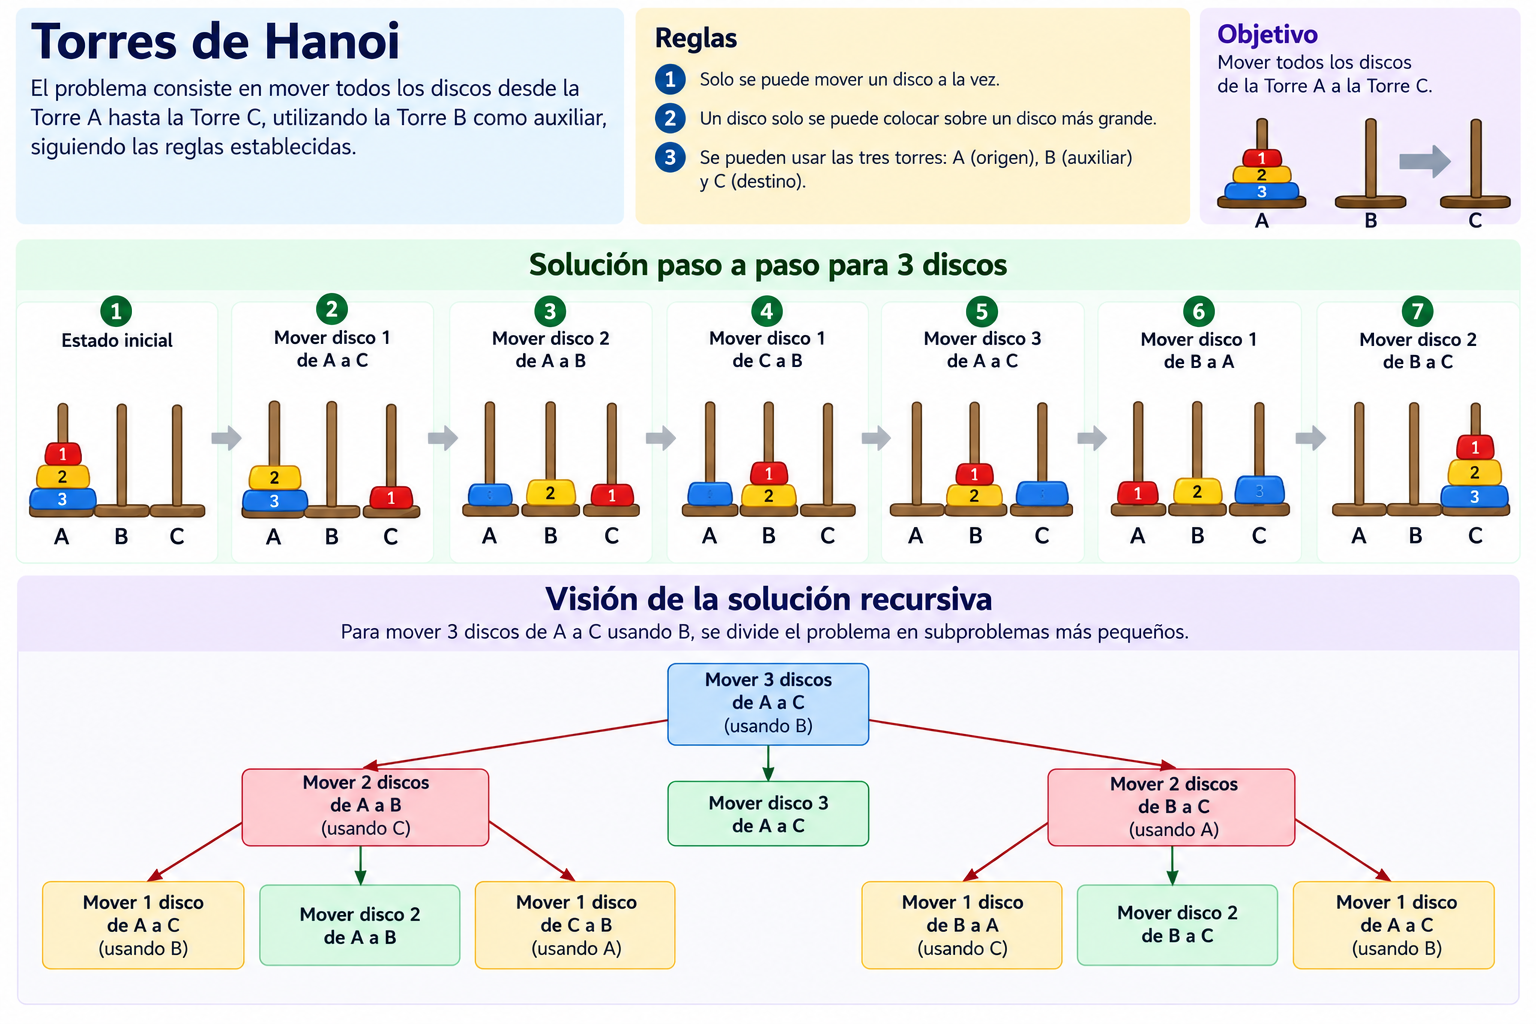
\includegraphics[width=\linewidth]{recursividad_torres_hanoi.png}
        \end{figure}
    \end{frame}

    \begin{frame}{Ventajas y desventajas}
        \begin{center}
            \footnotesize
            \begin{tabular}{@{}p{5.2cm}p{5.2cm}@{}}
                \toprule
                \textbf{Ventajas} & \textbf{Desventajas} \\
                \midrule
                Facilita la solución de problemas que pueden dividirse en subproblemas similares. &
                Cada llamada recursiva utiliza espacio en la pila de ejecución. \\
                Permite representar de forma natural estructuras jerárquicas y anidadas. &
                Puede resultar difícil seguir el orden de ejecución y retorno. \\
                Puede producir soluciones más simples y expresivas. &
                Puede repetir cálculos innecesarios si no se diseña adecuadamente. \\
                Favorece la descomposición de problemas complejos. &
                Python establece un límite de profundidad para las llamadas recursivas. \\
                \bottomrule
            \end{tabular}
        \end{center}
    \end{frame}

    \begin{frame}{Ventajas y desventajas}
        \begin{center}
            \footnotesize
            \begin{tabular}{@{}p{5.2cm}p{5.2cm}@{}}
                \toprule
                \textbf{Ventajas} & \textbf{Desventajas} \\
                \midrule
                Facilita la solución de problemas que pueden dividirse en subproblemas similares. &
                Cada llamada recursiva utiliza espacio en la pila de ejecución. \\
                Permite representar de forma natural estructuras jerárquicas y anidadas. &
                Puede resultar difícil seguir el orden de ejecución y retorno. \\
                Puede producir soluciones más simples y expresivas. &
                Puede repetir cálculos innecesarios si no se diseña adecuadamente. \\
                Favorece la descomposición de problemas complejos. &
                Python establece un límite de profundidad para las llamadas recursivas. \\
                \bottomrule
            \end{tabular}
        \end{center}
        \vspace{0.6em}
        {\scriptsize\color{green!40!black}\textbf{La recursividad puede simplificar la solución de problemas
        complejos, pero su uso debe considerar el consumo de memoria, la eficiencia y la claridad del algoritmo.}}
    \end{frame}

    \begin{frame}[fragile, t]{Ejercicios: Identificar componentes}
        \begin{minted}[xleftmargin=-2cm, frame=leftline, fontsize=\small]{python}
            def cuenta(n):
                if n == 0:
                    return

                print(n)
                cuenta(n-1)
        \end{minted}
    \end{frame}

    \begin{frame}[fragile, t]{Ejercicios: Identificar componentes}
        \begin{minted}[xleftmargin=-2cm, frame=leftline, fontsize=\small]{python}
            def cuenta(n):
                if n == 0:
                    return
                print(n)
                cuenta(n-1)
        \end{minted}
        \begin{itemize}
            \item ¿Cual es el caso base?
            \item ¿Cual es el caso recursivo?
            \item ¿Que sucede cuando n disminuye?
            \item ¿Que se imprime al ejecutar \mintinline{python}{cuenta(4)}?
        \end{itemize}
    \end{frame}

    \begin{frame}[fragile, t]{Ejercicios: Completar la función}
        \begin{minted}[xleftmargin=-2cm, frame=leftline, fontsize=\small]{python}
            def suma(n):
                if __________:
                    return 0

                return __________

            print(suma(5)) # Imprime 15
        \end{minted}
    \end{frame}

    \begin{frame}[fragile, t]{Ejercicios: Qué imprime la función?}
        \begin{minted}[xleftmargin=-2cm, frame=leftline, fontsize=\small]{python}
            def funcion(n):
                if n == 0:
                    return
                print(n)
                funcion(n - 1)
                print(n)

            funcion(3)
        \end{minted}
        Opciones:
        \begin{enumerate}
            \item 3 2 1
            \item 1 2 3
            \item 3 2 1 1 2 3
            \item 3 3 2 2 1 1
        \end{enumerate}
    \end{frame}

    \begin{frame}[fragile, t]{Ejercicios: Construir una pirámide recursiva}
        Desarrolla una función que reciba un número entero positivo n y construya una pirámide de asteriscos con n niveles.
        
        Por ejemplo, para n = 4, la función debe imprimir:
        \begin{verbatim}
               *
              ***
             *****
            *******
        \end{verbatim}

        \begin{itemize}
            \item No se pueden utilizar ciclos \mintinline{python}{for} o \mintinline{python}{while}.
            \item Se deben utilizar operaciones con strings.
            \item La función debe implementar un caso base y un caso recursivo.
        \end{itemize}
    \end{frame}

    \begin{frame}[fragile, t]{Ejercicios: Construir una pirámide recursiva}
        \begin{minted}[xleftmargin=-2cm, frame=leftline, fontsize=\small]{python}
            def piramide(n, nivel=1):
                espacios = " " * (n - nivel)
                estrellas = "*" * (2 * nivel - 1)
                fila = espacios + estrellas
                
                # Caso base
                if __________:
                    return fila
                else:
                    # Caso recursivo
                    return fila + "\n" + piramide(n, ______ + 1)

            print(piramide(4))
        \end{minted}
    \end{frame}

    \begin{frame}[fragile, t]{Ejercicios: Construir una pirámide invertida}
        Modifica el código para construir una pirámide invertida.
        Por ejemplo, para n = 4, la función debe imprimir:
        \begin{verbatim}
            *******
             *****
              ***
               *
        \end{verbatim}
        
    \end{frame}

    \begin{frame}{Ejercicios: Torres de Hanoi}
        Se dispone de tres torres: A, B y C. La torre A contiene n discos ordenados de mayor a menor tamaño.

        El objetivo es mover los n discos a la torre C, usando la torre B como auxiliar, siguiendo las siguientes reglas:
        \begin{itemize}
            \item Solo se puede mover un disco a la vez.
            \item No se puede colocar un disco grande encima de uno más pequeño.
            \item Solo se puede mover el disco que se encuentra en la parte superior de una torre.
        \end{itemize}
        
        Desarrollar una función recursiva que muestre los movimientos necesarios para resolver el problema.
        
    \end{frame}

    \begin{frame}{Ejercicios: Torres de Hanoi}
        \begin{figure}
            \centering
            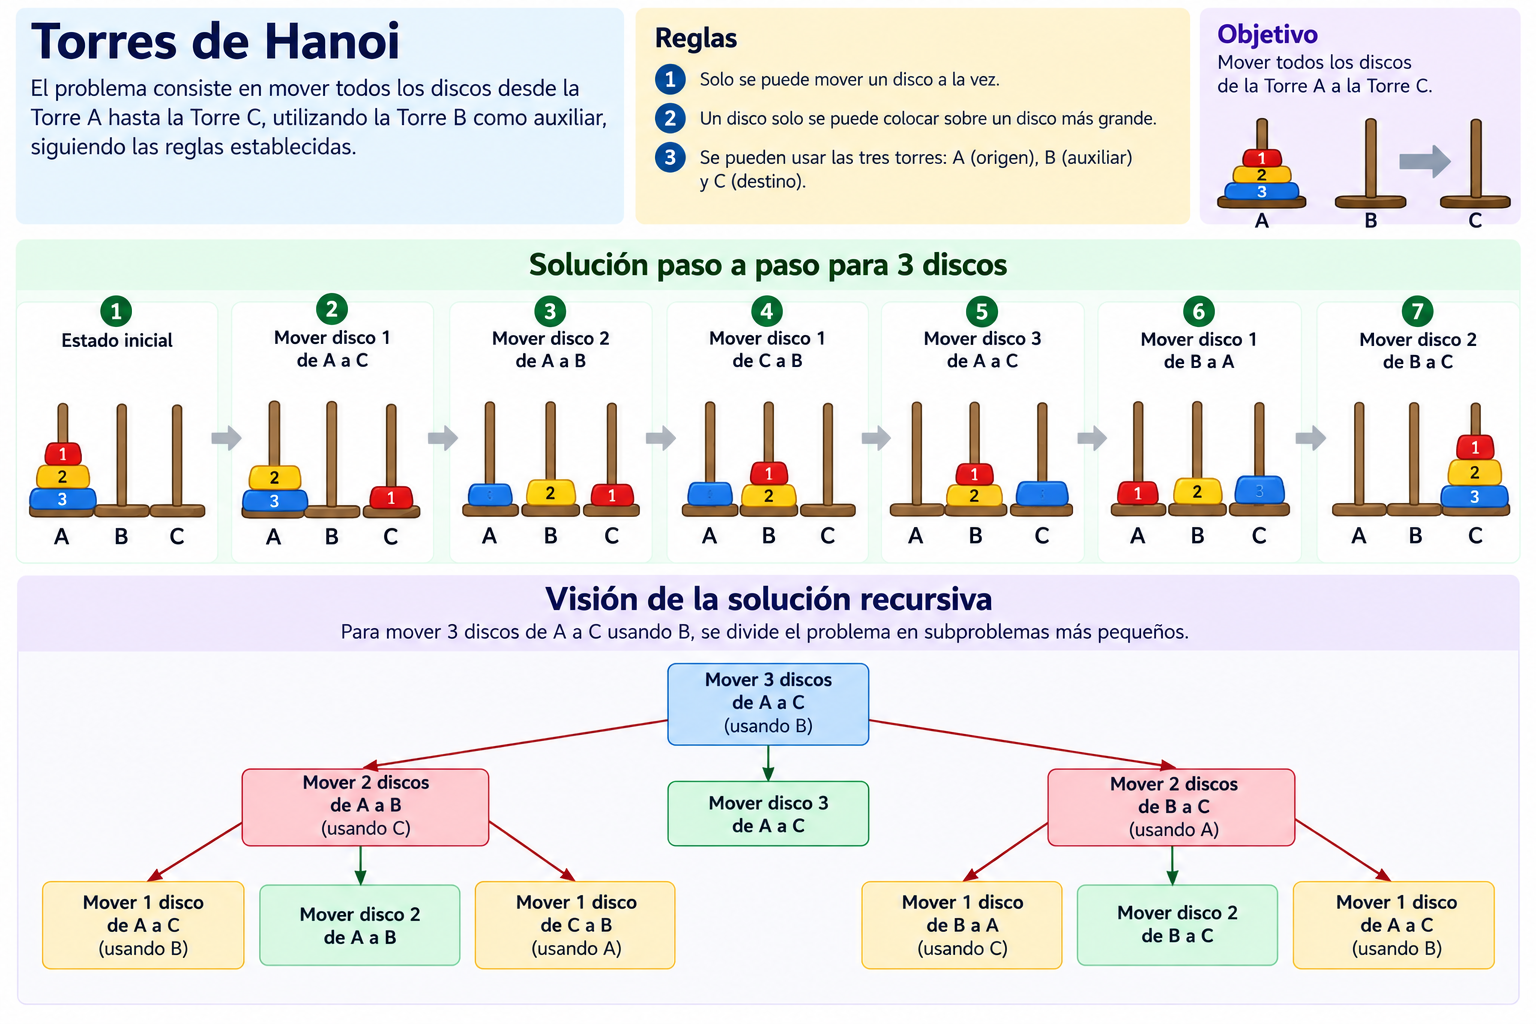
\includegraphics[width=\linewidth]{recursividad_torres_hanoi.png}
        \end{figure}
    \end{frame}

    \begin{frame}[fragile, t]{Ejercicios: Torres de Hanoi}
        Ejemplo para tres discos:
        \begin{minted}[xleftmargin=-2cm, frame=leftline, fontsize=\small]{python}
            hanoi(3, 'A', 'C', 'B')
            # Resultado:
            Mover disco de A a C
            Mover disco de A a B
            Mover disco de C a B
            Mover disco de A a C
            Mover disco de B a A
            Mover disco de B a C
            Mover disco de A a C
        \end{minted}
    \end{frame}

    \begin{frame}[fragile, t]{Ejercicios: Torres de Hanoi}
        \begin{minted}[xleftmargin=-2cm, frame=leftline, fontsize=\small]{python}
            def hanoi(n, origen, destino, auxiliar):
                # Caso base
                if __________:
                    print("Mover disco de", origen, "a", destino)
                    return

                hanoi(__________, origen, _______, destino)

                print("Mover disco de", origen, "a", destino)

                hanoi(n - 1, ________, destino, _______)
        \end{minted}
    \end{frame}

    \begin{frame}[fragile, t]{Ejercicios: Torres de Hanoi}
        \begin{minted}[xleftmargin=-2cm, frame=leftline, fontsize=\small]{python}
            def hanoi(n, origen, destino, auxiliar):
                # Caso base
                if n == 1:
                    print("Mover disco de", origen, "a", destino)
                    return

                # Mover n-1 discos hacia la torre auxiliar
                hanoi(__________, origen, ________, destino)

                # Mover el disco mas grande hacia el destino
                print("Mover disco de", origen, "a", destino)

                hanoi(n - 1, ________, destino, _______)
        \end{minted}
    \end{frame}

    \begin{frame}[fragile, t]{Ejercicios: Torres de Hanoi}
        \begin{minted}[xleftmargin=-2cm, frame=leftline, fontsize=\small]{python}
            def hanoi(n, origen, destino, auxiliar):
                # Caso base
                if n == 1:
                    print("Mover disco de", origen, "a", destino)
                    return

                # Mover n-1 discos hacia la torre auxiliar
                hanoi(n - 1, origen, auxiliar, destino)

                # Mover el disco mas grande hacia el destino
                print("Mover disco de", origen, "a", destino)

                hanoi(n - 1, ________, destino, _______)
        \end{minted}
    \end{frame}

    \begin{frame}[fragile, t]{Ejercicios: Torres de Hanoi}
        \begin{minted}[xleftmargin=-2cm, frame=leftline, fontsize=\small]{python}
            def hanoi(n, origen, destino, auxiliar):
                # Caso base
                if n == 1:
                    print("Mover disco de", origen, "a", destino)
                    return

                # Mover n-1 discos hacia la torre auxiliar
                hanoi(n - 1, origen, auxiliar, destino)

                # Mover el disco mas grande hacia el destino
                print("Mover disco de", origen, "a", destino)

                # Mover n-1 discos desde la torre auxiliar al destino
                hanoi(n - 1, auxiliar, destino, origen)
        \end{minted}
    \end{frame}

    \begin{frame}[fragile, t]{Ejercicios: Torres de Hanoi}
        El algoritmo de las Torres de Hanoi realiza exactamente:
        \begin{equation}
            M(n) = 2^{n} - 1
        \end{equation}
        movimientos necesarios para resolver el problema con \textit{n} discos.
    \end{frame}


    \begin{frame}{Resumen}
        \begin{itemize}
            \item La recursividad es una técnica de programación que permite resolver un problema mediante llamadas a una función que resuelve versiones más pequeñas del mismo problema.
            \pause
            \item Una función recursiva es una función que se llama a sí misma.
            \pause
            \item Una solución recursiva debe tener un caso base, un caso recursivo y garantizar el progreso hacia la terminación.
            \pause
            \item La recursividad e iteración permiten resolver problemas repetitivos, pero utilizan mecanismos de ejecución diferentes.
            \pause
            \item La recursividad puede simplificar la solución de problemas complejos, pero su uso debe considerar el consumo de memoria, la eficiencia y la claridad del algoritmo.
        \end{itemize}
    \end{frame}
\end{document}